\part{Back on Recursion}
\label{derecurs}\mypartpage
%%%%%%%%%%%%%%%%%%%%%%%%%%%%%%%%%%%%%%%%%%%%%%%%%%%%%%%%%%%%%%%%%%%%%%%%%%%%%%
\section{Avoiding Recursion}
\begin{frame}{Why do you want to avoid recursion}
  \begin{block}{What gets done on Function Calls}
    \begin{enumerate}
    \item Create a function frame on the stack
    \item Push (copy) value of parameters
    \item Execute function
    \item Pop return value
    \item Destruct stack frame
    \end{enumerate}
  \end{block}
  
  \begin{block}{Recursion does not interfere with this schema}
    \begin{itemize}
    \item Recursion can thus be less efficient than iterative solutions
    \item In time: function calling has a price
    \item In space: the call stack must be stored
    \end{itemize}
  \end{block}
\end{frame}
%%%%%%%%%%%%%%%%%%%%%%%%%%%%%%%%%%%%%%%%%%%%%%%%%%%%%%%%%%%%%%%%%%%%%%%%%%%%%%
\begin{frame}{Example: gcd of two natural integers}
  \concept{Greatest Common Divisor}\bigskip

  \begin{block}{gcd(a, b : Integer) = (r : Integer)}
    \begin{itemize}
    \item \structure{Precondition:} $a\geq b\geq  0$
    \item \structure{Postcondition:}
      $(a\text{ mod }r = 0)$ and $(b\text{ mod }r = 0)$ and
      $\neg\left(\exists s, (s > r)\wedge(a\text{ mod }s = 0)\wedge(b\text{ mod }s = 0)\right)$

    \end{itemize}
  \end{block}

  \begin{block}{Recursive Definition}\medskip
    \centerline{\fbox{\vbox{\vspace{-\baselineskip}%
        \begin{tabbing}%
          \textbf{if} $b = 0$ \=\textbf{then} \=$r\leftarrow a$\\
          \>\textbf{else}\>$r\leftarrow gcd(b, a\text{ mod }b)$
        \end{tabbing}\vspace{-\baselineskip}%
    }}}
  \end{block}
\end{frame}
%%%%%%%%%%%%%%%%%%%%%%%%%%%%%%%%%%%%%%%%%%%%%%%%%%%%%%%%%%%%%%%%%%%%%%%%%%%%%%
\begin{frame}{Computation of gcd(420,75)}
    \centerline{\fbox{\vbox{\vspace{-\baselineskip}%
        \begin{tabbing}%
          \textbf{if} $b = 0$ \=\textbf{then} \=$r\leftarrow a$\\
          \>\textbf{else}\>$r\leftarrow gcd(b, a\text{ mod }b)$
        \end{tabbing}\vspace{-\baselineskip}%
    }}}
  \vspace{-\baselineskip}
  \begin{columns}
    \begin{column}{.2\linewidth}
      \includegraphics<11,12| handout:0>[subfig=6]{fig/rec_pgcd_exemple.fig}%    
      \includegraphics<1,10| handout:0>[subfig=1]{fig/rec_pgcd_exemple.fig}%    
      \includegraphics<2,9| handout:0>[subfig=2]{fig/rec_pgcd_exemple.fig}%    
      \includegraphics<3,8| handout:0>[subfig=3]{fig/rec_pgcd_exemple.fig}%    
      \includegraphics<4,7| handout:0>[subfig=4]{fig/rec_pgcd_exemple.fig}%    
      \includegraphics<5,6| handout:1>[subfig=5]{fig/rec_pgcd_exemple.fig}%    
    \end{column}%
    \begin{column}{.8\linewidth}
      \begin{minipage}{.6\linewidth}
        \begin{itemize}
        \item $gcd(420,75) =\uncover<2->{gcd(75,45)
            \visible<11->{\boldsymbol{=15}}$
          \item $gcd(75,45) = }\uncover<3->{gcd(45,30)
            \visible<10->{\boldsymbol{=15}}$
          \item $gcd(45,30) = }\uncover<4->{gcd(30,15)
            \visible<9->{\boldsymbol{=15}}$
          \item $gcd(30,15) = }\uncover<5->{gcd(15,0)
            \visible<8->{\boldsymbol{=15}}$
          \item $gcd(15,0)  = }$\uncover<6->{15 \\
            \alert{this is the Base Case}}
        \end{itemize}
      \end{minipage}\begin{minipage}{.4\linewidth}
        \centerline{\visible<12->{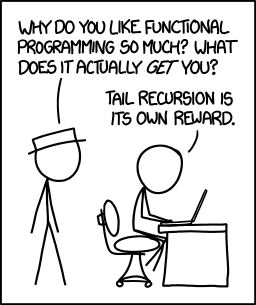
\includegraphics[width=.7\linewidth]{img/xkcd-functional.png}%
          {\tiny~}%
          \rotatebox{90}{\tiny\url{http://xkcd.com/1270/}}}}
      \end{minipage}
      \begin{itemize}
      \uncover<7->{
        \item Let's pop parameters
        \item $r\leftarrow r_{int}$ (no other computation:
        $G(x,y)=y$)} 
      \bigskip
      \uncover<11->{\item The result of initial call is known as early as from 
        Base Case\\ 
        {\large This is known as \alert{\textbf{Tail Recursion}}}}
      \visible<12->{\item Factorial: multiplications during climb up\\
      $\Rightarrow$ \textbf{non-terminal} recursion}
      \end{itemize}
    \end{column}
  \end{columns}
\end{frame}
%%%%%%%%%%%%%%%%%%%%%%%%%%%%%%%%%%%%%%%%%%%%%%%%%%%%%%%%%%%%%%%%%%%%%%%%%%%%%%
\begin{frame}{Transformation to Non-Recursive Form}
  \concept{Every recursive function can be changed to a non-recursive form}
  \bigskip\bigskip

  \large
  Several Methods depending on function:
  \begin{itemize}
  \item \structure{Tail Recursion}: very simple transformation
  \item \structure{Non-Tail Recursion}: two methods (only one is generic)
  \end{itemize}
    \bigskip
  
  Compilers use these optimization techniques
  {\normalsize (amongst much others)}
\end{frame}
%%%%%%%%%%%%%%%%%%%%%%%%%%%%%%%%%%%%%%%%%%%%%%%%%%%%%%%%%%%%%%%%%%%%%%%%%%%%%%
\subsection{Non-Recursive Form of Tail Recursion}
\begin{frame}{Non-Recursive Form of Tail Recursion}
  \begin{block}{Cookbook to change Tail Recursion to Non-Recursive Form}
    
  \begin{itemize}
  \item Generic \structure{recursive algorithm} ~~~~~~~~~
    \uncover<3->{\structure{Example:} get last char of string}
    \begin{columns}
      \fbox{\begin{column}{.45\linewidth}\vspace{-.4\baselineskip}
        \begin{tabbing}%
          $f(x)$:\\
          ~~\textbf{if} cond(x) \=\textbf{then} \=\textsc{BaseCase}(x)\\
          \>\textbf{else}\>\textsc{t}(x); $r\leftarrow f(x_{int})$
        \end{tabbing}
      \end{column}}

    \uncover<3->{
    \fbox{\begin{column}{.5\linewidth}\vspace{-.4\baselineskip}
        \begin{tabbing}%
          last(s):\\
          ~~\textbf{if} empty(cdr(s)) \=\textbf{then} \=$r\leftarrow car(s)$\\
          \>\textbf{else} \> $r\leftarrow last(cdr(s))$
        \end{tabbing}
    \end{column}}}
    \begin{column}{.001\linewidth}~\end{column}
  \end{columns}
  \bigskip
  
  \uncover<2->{
  \item Equivalent \structure{iterative algorithm}
    \begin{columns}
      \fbox{\begin{column}{.45\linewidth}\vspace{-.4\baselineskip}
        \begin{tabbing}%
          $f'(x)$:\\
          ~~\= $u\leftarrow x$\\
          \>\textbf{until} cond(u) \=\textbf{do}\\
          \>~~\=T(u)\\
          \>\>$u\leftarrow h(u)$\\
          \>\textbf{end}\\
          \>\textsc{BaseCase}(u)
        \end{tabbing}
      \end{column}}

    \uncover<4->{
    \fbox{\begin{column}{.5\linewidth}\vspace{-.4\baselineskip}
        \begin{tabbing}%
          last'(s):\\
          ~~$l \leftarrow s$\\
          ~~\textbf{until} $empty(cdr(l))$  \textbf{do}\\
          ~~~~\textit{// T(u) does nothing }\\
          ~~~~\=l=cdr(l)\\
          ~~\textbf{end} \\
          ~~$r\leftarrow car(l)$
        \end{tabbing}
    \end{column}}}
    \begin{column}{.001\linewidth}~\end{column}
  \end{columns}
}

  \end{itemize}
  \end{block}
\end{frame}
%%%%%%%%%%%%%%%%%%%%%%%%%%%%%%%%%%%%%%%%%%%%%%%%%%%%%%%%%%%%%%%%%%%%%%%
\begin{frame}[fragile]{Other Examples}
  \begin{block}{nth(s,i): get char number $i$ out of $s$}
    \begin{columns}\medskip
      \begin{column}{.45\linewidth}
        \fbox{\begin{minipage}{\linewidth}
            \begin{tabbing}%
              nth(s,i):\\
              ~~\textbf{if} n=0 \=\textbf{then} \=$r\leftarrow car(s)$\\
              \>\textbf{else} \> $r\leftarrow nth(cdr(s),i-1)$
            \end{tabbing}
        \end{minipage}}
      
      \bigskip
      Two arguments, still no T(u)
      \end{column}
      
      \uncover<2->{
      \begin{column}{.4\linewidth}
        \fbox{\begin{minipage}{\linewidth}
            \begin{tabbing}%
              nth'(s,i):\\
              ~~$l \leftarrow s$; $k\leftarrow i$\\
              ~~\textbf{until} k=0 \textbf{do}\\
              ~~~~\=l=cdr(l); k=k-1\\
              ~~\textbf{end} \\
              ~~$r\leftarrow car(l)$
            \end{tabbing}
          \end{minipage}}
      \end{column}}
    \end{columns}
  \end{block}
  
  \begin{block}<3->{is\_member(s,c): assess whether $c$ is member of $s$}
    \begin{columns}\medskip
      \begin{column}{.5\linewidth}
        \fbox{\begin{minipage}{\linewidth}
            \begin{tabbing}%
              is\_member(s,c):\\
              ~~\textbf{if} empty(s) \textbf{then} \=$r\leftarrow FALSE$\\
              ~~\textbf{if} car(s)=c \=\textbf{then} \= $r\leftarrow TRUE$\\
              \>\textbf{else}\>$r\leftarrow is\_memb(cdr(s))$
            \end{tabbing}
        \end{minipage}}
      
      \bigskip
      \hbox{2 base cases, still no T(u)}
      \end{column}

      \uncover<4->{
      \begin{column}{.4\linewidth}
        \fbox{\begin{minipage}{\linewidth}
            \begin{tabbing}%
              is\=\_memb'(s,c):\\
              ~~$l \leftarrow s$\\
              ~~\textbf{until} $empty(l)$ OR car(l)=c \textbf{do}\\
              ~~~~\=l=cdr(l)\\
              ~~\textbf{end} \\
              ~~\textbf{if} empty(s) \textbf{then} \=$r\leftarrow FALSE$\\
              ~~$r\leftarrow TRUE$
            \end{tabbing}
          \end{minipage}}
      \end{column}}
    \end{columns}
  \end{block}
\end{frame}
%%%%%%%%%%%%%%%%%%%%%%%%%%%%%%%%%%%%%%%%%%%%%%%%%%%%%%%%%%%%%%%%%%%%%%%%%%%%%%
\begin{frame}{Last Example}
  \begin{block}{Non-Recursive Form of GCD}
    \begin{columns}
      \begin{column}{.48\linewidth}
        \centerline{\fbox{\vbox{\vspace{-\baselineskip}%
              \begin{tabbing}%
                $gcd(a,b)$:\\
                ~~\textbf{if} $b = 0$ \=\textbf{then} \=$r\leftarrow a$\\
                \>\textbf{else}\>$r\leftarrow gcd(b, a\text{ mod }b)$
              \end{tabbing}\vspace{-\baselineskip}%
            }}}
      \end{column}

    % \uncover<2->{
    % \begin{column}{.52\linewidth}
    %   \begin{description}
    %   \item[cond(a,b):] b=0
    %   \item[\textsc{BaseCase}(a,b):] $r\leftarrow a$
    %   \item[\textsc{GenCase}(a,b):] \textsc{t}(a,b); $r\leftarrow
    %     gcd(a_{int},b_{int})$
    %   \item[\textsc{t}(a,b):] $ a_{int}\leftarrow b$
    %   \item[] $b_{int}\leftarrow a\text{ mod }b$
    %   \end{description}\end{column}
    % }

      \fbox{\begin{column}{.3\linewidth}\vspace{-\baselineskip}
        \begin{tabbing}%
          $gcd'(a,b)$:\\
          ~~\= $u\leftarrow a$; $v\leftarrow b$\\
          \>\textbf{until} v=0 \=\textbf{do}\\
          \>~~\=$temp\leftarrow v$\\
          \>\>$v\leftarrow u\text{ mod }v$\\
          \>~~\=$u\leftarrow temp$\\
          \>\textbf{end}\\
          \>$r\leftarrow u$
        \end{tabbing}
      \end{column}}

    \begin{column}{.001\linewidth}~\end{column}
  \end{columns}
  \end{block}

  \begin{itemize}
  \item This is given by an immediate rewriting
  \item Computers are good at this kind of game (ie compilers)
  \item Meta-programming troubling at first sight, but still fully mechanic
  \end{itemize}
\end{frame}
%%%%%%%%%%%%%%%%%%%%%%%%%%%%%%%%%%%%%%%%%%%%%%%%%%%%%%%%%%%%%%%%%%%%%%%%%%%%%%
\subsection{Transformation to Tail Recursion}
\begin{frame}{Non-Recursive form of Non-Tail functions}
  \begin{block}{Previous approach is not often applicable}
  \begin{itemize}
  \item If the function you consider is non-tail, this method does not apply
  \item Looking closer, that's because of those computations at recursive
    climb:
  \item Where should the \structure{ongoing computation} be stored (they were stacked)?
    
    $fact(3)=\alert{3\times} fact(2)=\alert{3\times 2\times}
    fact(1)=\alert{3\times 2\times} 1=\alert{3\times} 2=6$ 
  \end{itemize}
\end{block}\vspace{-.7\baselineskip}
\begin{block}{What's done is no more to be done}
  \begin{itemize}
  \item Do intermediate computations during descent, not waiting for climbing\\[2pt]

    $fact(3)=\fbox{\alert{3}}\times fact(2)=\alert{3\times 2}\times
    fact(1)=\fbox{\alert{6}}\times fact(1)=\fbox{\alert{6}}\times
    1=\fbox{6}=6$\\[2pt]
    There's nothing left to do during climbing $\Rightarrow$ Tail Recursion

  \item One extra variable is enough for the storage of ``ongoing'' computation
    \begin{itemize}
    \item Since these computations are done, store their result not the
      stack of operations
    \item Adding an extra parameter to my recursive function does the trick
    \item Prototype change $\leadsto$ put recursion into a \textit{helper}
      function with more parameters
    \end{itemize}
  \end{itemize}
\end{block}\vspace{-.7\baselineskip}

\begin{block}{\alert{Warning:} this does not always work!}
  \begin{itemize}
  \item Computations done out of order $\leadsto$ must be \alert{associative}
    and \alert{commutative}
  \item This (simple) method does not always work; another one comes afterward
  \end{itemize}
  \end{block}
\end{frame}
%%%%%%%%%%%%%%%%%%%%%%%%%%%%%%%%%%%%%%%%%%%%%%%%%%%%%%%%%%%%%%%%%%%%%%%%%%%%%%
\begin{frame}{Example: Changing Factorial into Tail Recursion}

  \begin{columns}
    \begin{column}{.45\linewidth} 
    \fbox{\vbox{\vspace{-.8\baselineskip} %
        \begin{tabbing}%
          \textsc{fact}(n):\\
          ~~\textbf{if} n = 0 \=\textbf{then} \=$r\leftarrow 1$ \\
          \> \textbf{else} \>$r\leftarrow n\times fact(n-1)$
        \end{tabbing}\vspace{-.8\baselineskip}%
      }
    }         
    \end{column}
    \begin{column}{.5\linewidth} 
    \fbox{\vbox{\vspace{-.8\baselineskip} %
        \begin{tabbing}%
          \uncover<2->{\alert<2| handout:0>{\textsc{fact'}(n): $\lambda(n,1)$}}\\
          \alert<1| handout:0>{$\lambda(n,acc):$}\\
          \uncover<3->{~~\textbf{if} n = 0 \uncover<4->{ \=\textbf{then} \=
              \alert<4| handout:0>{$r\leftarrow acc$}} \\
            \> \textbf{else} \>\alert<3| handout:0>{$r\leftarrow \lambda(n-1, acc\times n)$}}
        \end{tabbing}\vspace{-.8\baselineskip}%
      }
    }         
    \end{column}
  \end{columns}


  \begin{block}{Step-by-step approach}
    \begin{enumerate}
    \item[0.] (it works because the addition is commutative and associative)
    \item Create a lambda function doing the recursion, with more parameters
      \begin{itemize}
      \item Local copy of the parameters carrying the recursion
      \item Add as many accumulators as operations done on climb up
      \end{itemize}
    \item<2-> Main function simply calls the lambda function
      \begin{itemize}
      \item Copy of the parameters carrying the recursion
      \item Initialize accumulators to the identity element of their operation
      \end{itemize}
    \item<3-> Body of the lambda function:
      \begin{itemize}
      \item General treatment: as before, but do intermediate ops into the accumulators
      \item<4-> Base case: get result directly from the accumulators
      \end{itemize}
    \end{enumerate}
  \end{block}
\end{frame}
%%%%%%%%%%%%%%%%%%%%%%%%%%%%%%%%%%%%%%%%%%%%%%%%%%%%%%%%%%%%%%%%%%%%%%%%%%%%%%
\begin{frame}{Let's take another example}
  \begin{block}{Computation of a string's length}\medskip
    \begin{columns}
      \begin{column}{.48\linewidth}
        \fbox{\vbox{\vspace{-.7\baselineskip}\begin{tabbing}
          len(str):\\
          ~~\textbf{if} empty(s) \=\textbf{then} \=0\\
          \>\textbf{else} \>\alert<1| handout:0>{1+}len(cdr(s))
        \end{tabbing}\vspace{-.7\baselineskip}}}
      \end{column}

      \begin{column}{.48\linewidth}
        \fbox{\vbox{\vspace{-.7\baselineskip}\begin{tabbing}
          \uncover<2->{\alert<2| handout:0>{len'(str) = $\lambda$(str,0)}}\\[5pt]
          \alert<1| handout:0>{$\lambda$(str,acc):} \\
          \uncover<3->{~~\textbf{if} empty(str) 
            \uncover<4->{\=\textbf{then} \= \alert<4| handout:0>{acc}}\\
          \>\textbf{else} \>\alert<3| handout:0>{$\lambda$(cdr(str), acc+1)}}
        \end{tabbing}\vspace{-.7\baselineskip}}}
      \end{column}
    \end{columns}
  \end{block}

  \begin{enumerate}
  \item[0.] (works because addition is commutative and associative)
  \item Create a $\lambda$ function doing the recursion, adding one accumulator
    per operation
  \item<2-> Main function: calls the lambda function and initializes the parameters
  \item<3-> Body of the $\lambda$ function:
    \begin{itemize}
    \item General treatment: as before, but do intermediate ops into the accumulator(s)
    \item<4-> Base case: get result directly from the accumulator(s)
    \end{itemize}
  \end{enumerate}
\end{frame}
%%%%%%%%%%%%%%%%%%%%%%%%%%%%%%%%%%%%%%%%%%%%%%%%%%%%%%%%%%%%%%%%%%%%%%%%%%%%%%
\begin{frame}{Closing the loop: Non-recursive form of Factorial}
  \begin{columns}
    \begin{column}{.45\linewidth} 
    \fbox{\vbox{\vspace{-.8\baselineskip} %
        \begin{tabbing}%
          \textsc{fact}(n):\\
          ~~\textbf{if} n = 0 \=\textbf{then} \=$r\leftarrow 1$ \\
          \> \textbf{else} \>$r\leftarrow n\times fact(n-1)$
        \end{tabbing}\vspace{-.8\baselineskip}%
      }
    }         
    \end{column}
    \begin{column}{.5\linewidth} 
    \fbox{\vbox{\vspace{-.8\baselineskip} %
        \begin{tabbing}%
          \textsc{fact'}(n): $\lambda(n,1)$\\
          $\lambda(n,acc):$\\
          ~~\textbf{if} n = 0 \=\textbf{then} \= $r\leftarrow acc$ \\
          \> \textbf{else} \>$r\leftarrow \lambda(n-1, acc\times n)$
        \end{tabbing}\vspace{-.8\baselineskip}%
      }
    }         
    \end{column}
  \end{columns}

  \begin{itemize}
  \item This function uses Tail Recursion
  \item[$\leadsto$] We can turn the helper into non-recursion with the method seen  before
  \item<3-> Then, we combine everything
  \end{itemize}

  \begin{columns}
    \uncover<2->{
    \begin{column}{.45\linewidth} 
    \fbox{\vbox{\vspace{-.8\baselineskip} %
        \begin{tabbing}%
          $\lambda'(n,acc):$\\
          ~~\=$td\leftarrow n$; $a\leftarrow acc$\\
          \>\textbf{until} $td=0$ \textbf{do}\\
          \>~~\=$a\leftarrow a\times td$
                            \hspace{4mm}\=\structure{// beware of the }\\
          \>\>$td\leftarrow td-1$\>\structure{// updates' order }\\
          \>\textbf{end}\\
          \>return $a$
        \end{tabbing}\vspace{-\baselineskip}%
      }}
    \end{column}}

    \uncover<3->{
    \begin{column}{.45\linewidth} 
    \fbox{\vbox{\vspace{-.8\baselineskip} %
        \begin{tabbing}%
          \alert{\textsc{fact}''(n)}:\\
          ~~\=$td\leftarrow n$; $a\leftarrow \alert{1}$\\
          \>\textbf{until} $td=0$ \textbf{do}\\
          \>~~\=$a\leftarrow a\times td$\\
          \>\>$td\leftarrow td-1$\\
          \>\textbf{end}\\
          \>return $a$
        \end{tabbing}\vspace{-\baselineskip}%
      }}
    \end{column}}
  \end{columns}
  \begin{itemize}
  \item<3-> These two transformations are simple, automatic and neat\ldots
  \item<4-> \ldots when applicable!!! \Frownie ~~~If not, let's get angry and mean!
  \end{itemize}

\end{frame}

%%%%%%%%%%%%%%%%%%%%%%%%%%%%%%%%%%%%%%%%%%%%%%%%%%%%%%%%%%%%%%%%%%%%%%%%%%%%%%
\subsection{Generic Algorithm Using a Stack}
\begin{frame}{Generic Algorithm Using a Stack}
  \begin{block}{Idea}
  \begin{itemize}
  \item Processors are sequential and execute any recursive function \\
   \textit{$\Rightarrow$ Always possible to express without recursion}
  \item \structure{Principle:} simulating the function stack of processors\\
    \alert{\textbf{By using a stack explicitly}}
    \pause
  \end{itemize}    
  \end{block}\vspace{-.7\baselineskip}

  \begin{block}{Example with only one recursive call}\vspace{-2\baselineskip}
    \begin{columns}
    \begin{column}[b]{.5\linewidth}    
        \centerline{\fbox{\vbox{\vspace{-\baselineskip} %
            \begin{tabbing}%
            \textbf{if} cond(x) \=\textbf{then} \=$r\leftarrow g(x)$ \\
            \> \textbf{else} \>\textsc{t}(x); $r\leftarrow G(x,f(x_{int}))$
          \end{tabbing}\vspace{-\baselineskip}%
        }}}
      \visible<4->{
      \bigskip
      
        \structure{Remark:}\\
        If $h()$ is invertible, no need for a stack:\\
        parameter reconstructed by $h^{-1}()$\\[.5\baselineskip]
        Stopping Condition = counting calls

      }
    \end{column}
    \pause
    \begin{column}[b]{.5\linewidth}    
        \centerline{\fbox{\vbox{\vspace{-\baselineskip} %
            \begin{tabbing}%
            $p\leftarrow emptyStack$\\
            $a\leftarrow x$ \structure{(* a: locale variable *)}\\
            \structure{(* pushing on stack (\alert{descent}) *)}\\
            \textbf{until} cond(a) \textbf{do}\\
            ~~\=push(p, a)\\
            \>$a\leftarrow h(a)$\\
            \textbf{end}\\
            $r\leftarrow g(a)$ \structure{(* Base Case *)} \\
            \structure{(* poping from stack (\alert{climb up}) *)}\\
            \textbf{until} stackIsEmpty(p) \textbf{do}\\
            \>$a\leftarrow top(p)$; pop(p); \textsc{t}(a)\\
            \>$r\leftarrow G(a,r)$\\
            \textbf{end}
          \end{tabbing}\vspace{-\baselineskip}%
        }}}
    \end{column}
  \end{columns}
\end{block}
\end{frame}
%%%%%%%%%%%%%%%%%%%%%%%%%%%%%%%%%%%%%%%%%%%%%%%%%%%%%%%%%%%%%%%%%%%%%%%%%%%%%%
\begin{frame}{Non-Recursive Form of Hanoï Towers (1/2)}
  \centerline{\fbox{\vbox{\vspace{-.8\baselineskip} %
    \begin{tabbing}%
    \textsc{hanoi}(n,a,b,c): \textit{(a to b, with c as disposal)}\\
      ~~\textbf{if} $n>0$ \textbf{then} \=hanoi(n-1, a, c)\\
                                        \>move(a, b)\\
                                        \>hanoi(n-1, c, b)
    \end{tabbing}\vspace{-.8\baselineskip}%
  }}}\medskip

  \begin{block}{One should mimic processor behavior wrt stacking}
    \begin{itemize}
    \item H(4,a,b,c) = \structure<1>{\alert<2>{H(3,a,c,b)}+D(a,b)+H(3,c,b,a)}
    \item<2-> Compute first unknown term:\hfill
              \alert<2>{H(3,a,c,b)} = \structure<2>{\alert<3>{H(2,a,b,c)}+D(a,c)+H(2,b,c,a)}
    \item<3-> Compute first unknown term:\hfill
              \alert<3>{H(2,a,b,c)} = \alert<4>{H(1,a,c,b)}+\structure<3>{D(a,b)}+\alert<5>{H(1,c,b,a)}
    \item<4-> Compute first unknown term:\hfill
              \alert<4>{H(1,a,c,b)} = \structure<4>{D(a,c)}
    \item<5-> Take on something casted aside:\hfill
              \alert<5>{H(1,c,b,a)} = \structure<5>{D(c,b)}
    \item<6-> and so on until everything casted aside is done (until stack
      is empty)
    \end{itemize}
  \end{block}\vspace{-.7\baselineskip}
  \begin{block}{We get:}\medskip
  H(4,a,b,c) = \uncover<4->{\structure<4>{D(a,c)}}%
               \uncover<3->{+\structure<3>{D(a,b)}+}%
               \uncover<5->{\structure<5>{D(c,b)}}%
               \uncover<2->{+\structure<2>{D(a,c)+H(2,b,c,a)}}+%
               \structure<1>{D(a,b)+H(3,c,b,a)}

  \uncover<2->{\vspace{-.5\baselineskip}              
  $\qquad\qquad\qquad\underbrace{\qquad\qquad\qquad\qquad\:\quad}$

  $\qquad\qquad\qquad\qquad\:$\structure<2>{H(2,a,b,c)}}

  \vspace{-.7\baselineskip}              
  $\qquad\qquad\qquad\underbrace{\quad\qquad\qquad\qquad\qquad\qquad\qquad\qquad\qquad\:\quad}$

  $\qquad\qquad\qquad\qquad\qquad\qquad\:$\structure<1>{H(3,a,c,b)}
  \end{block}
\end{frame}
%%%%%%%%%%%%%%%%%%%%%%%%%%%%%%%%%%%%%%%%%%%%%%%%%%%%%%%%%%%%%%%%%%%%%%%%%%%%%%
\newcommand{\etape}[1]{\multicolumn{1}{c}{\structure{Step #1}}}
\begin{frame}{Non-Recursive Form of Hanoï Towers (2/2)}
  \begin{flushright}
  \fbox{\vbox{\vspace{-.8\baselineskip} %
    \begin{tabbing}%
    \textsc{hanoi}(n,a,b):\\
      ~~\textbf{if} $n>0$ \textbf{then} \=hanoi(n-1, a, c)\\
                                        \>move(a, b)\\
                                        \>hanoi(n-1, c, b)
    \end{tabbing}\vspace{-.8\baselineskip}%
  }}
  \end{flushright}\vspace{-6\baselineskip}

  \begin{block}{hanoi\_derec(n, A, B) :}\vspace{-.8\baselineskip}
    {\small%
      \begin{tabbing}
        ~~~\=push (n, A, B, 1) on stack\\
        \>while (stack non-empty) \\
        \>~~~\=(n, A, B, CallKind) $\leftarrow$ pop()\\
        \>\>if ($n>0$)\\
        \>\>~~~\=if (CallKind == 1) \\
        \>\>\>~~~\=push (n, A, B, 2) on stack 
                   \structure{(* Cast something aside for later *)}\\
        \>\>\>\>push (n-1, A, C, 1) 
                   \structure{(* Compute first unknown soon *)}\\
        \>\>\>else /* ie, CallKind == 2 */\\
        \>\>\>\>move(A, B)\\
        \>\>\>\>push (n-1, C, B, 1) on stack\\
      \end{tabbing}
    }
  \end{block}\vspace{-2\baselineskip}

  \visible<2->{
  \resizebox{\linewidth}{!}{
  \begin{tabular}{cccccccccc}
                     &                  &                  &                  &\visible<6->{0AB1}&                   &                   &                  &&\\
                     &                  &                  &\visible<5->{1AC1}&\visible<6->{1AC2}&\visible<7->{0BC1} &                   &\visible<9->{0AB1}&&\\
                     &                  &\visible<4->{2AB1}&\visible<5->{2AB2}&\visible<6->{2AB2}&\visible<7->{2AB2} &\visible<8->{1CB1} &\visible<9->{1CB2}&\visible<10->{0AB1}&\\
                     &\visible<3->{3AC1}&\visible<4->{3AC2}&\visible<5->{3AC2}&\visible<6->{3AC2}&\visible<7->{3AC2} &\visible<8->{3AC2} &\visible<9->{3AC2}&\visible<10->{3AC2}&\visible<11->{2BC1}\\
   \visible<2->{4AB1}&\visible<3->{4AB2}&\visible<4->{4AB2}&\visible<5->{4AB2}&\visible<6->{4AB2}&\visible<7->{4AB2} &\visible<8->{4AB2} &\visible<9->{4AB2}&\visible<10->{4AB2}&\visible<11->{4AB2}\\
   \etape{1}         &\etape{2}         &\etape{3}         &\etape{4}         &\etape{5}         &\etape{6}          &\etape{8}          &\etape{9}         &\etape{11}         &\etape{13}\\
  \end{tabular}}
  hanoi(4,a,b)=\only<7->{D(ac)+}\only<8->{D(ab)+}\only<10->{D(cb)+}\only<11->{D(ac)+}\ldots}

  \medskip
  \uncover<12->{\structure{Rq:} simpler iterative algorithms exist 
    (they are not automatic transformations)\\
    {\footnotesize J.C. Fournier. 
      \textit{Pour en finir avec la dérécursivation du problème des tours de  Hanoï.}
    1990.}\\[-.5\baselineskip]
    {\tiny\url{http://archive.numdam.org/article/ITA_1990__24_1_17_0.pdf}}
}
\end{frame}
%%%%%%%%%%%%%%%%%%%%%%%%%%%%%%%%%%%%%%%%%%%%%%%%%%%%%%%%%%%%%%%%%%%%%%%%%%%%%%
\section{Back-tracking}
\sectionpage
%%%%%%%%%%%%%%%%%%%%%%%%%%%%%%%%%%%%%%%%%%%%%%%%%%%%%%%%%%%%%%%%%%%%%%%%%%%%%%
\begin{frame}{Combinatorial Search and Optimization}
  \concept{Large class of Problems with similar algorithmic approach}

  \begin{itemize}
  \item Solutions are really numerous; A set of constraints make some solution invalids
  \item \structure{Combinatorial Search} $\leadsto$ look for any valid solution\\
    \structure{Combinatorial Optimization} $\leadsto$ look for the solution
    maximizing a function
  \end{itemize}

  \begin{block}{Examples}
    \begin{itemize}
    \item \structure{Open the lock}: Find the right 4-digits combination out of 10000
    \item \structure{Knapsac}: Ali-Baba searches object set fitting in bag
      maximizing the value
    \item \structure{Minimum Spanning Tree} of a given graph
    \item \structure{Traveling Salesman:} visit $n$ cities in order minimizing
      the total distance
%    \item \structure{Artificial Intelligence:} select best solution from set of
%      possibilities 
    \end{itemize}
  \end{block}\vspace{-.7\baselineskip}

  \begin{block}{First Resolution Approach: Exhaustive Search}
    \begin{itemize}
    \item Study \textit{every} solutions\\
      {\small $\leadsto$ Test all lock combinations\\
        $\leadsto$ Enumerate all possible knapsack contents + get max value}
    \item This often reveals to be exponential and thus infeasible
    \end{itemize}
  \end{block}
\end{frame}
%%%%%%%%%%%%%%%%%%%%%%%%%%%%%%%%%%%%%%%%%%%%%%%%%%%%%%%%%%%%%%%%%%%%%%%%%%%%%%
\begin{frame}{Better Approach?}
  \begin{block}{Guessing the right number can become difficult that way}
    \begin{itemize}
    \item 
      $0001 \leadsto no$; $0002 \leadsto no$; $0003 \leadsto no$; 
      $0004 \leadsto no$; $0005 \leadsto no$; Booooring
    \item Let's more information: length of correct suffix instead of yes/no answers\\
      $0001 \leadsto 0$; $0002 \leadsto 0$; $000\alert{3} \leadsto 1$;
      $00\alert{24} \leadsto 2$; $0\alert{424} \leadsto 3$; $\alert{5424} \leadsto 4, bingo$
    \end{itemize}   
  \end{block}\vspace{-.6\baselineskip}
  \begin{block}<2->{This leads to a much more efficient algorithm:}
    \begin{itemize}
    \item Guess each position by testing every digit in that pos until response
      increases
    \item \uncover<3->{That's even
        easy to write by mixing recursion with a for loop:\\\smallskip
      \fbox{\hspace{-7mm}\vbox{\vspace{-.7\baselineskip}\begin{tabbing}
        search(current,pos,len): // initial values: search(\{0,0,0,0\}, 0, 0)\\
        ~~\textbf{for} $n\in[0;9]$ \textbf{do}\\
        ~~~~put $n$ into $current$ at position $pos$\\
        ~~~~\textbf{if} $try(current)>len$ \=\textbf{then} search(current,pos+1, try(current))\\
        \>\textbf{else} // no luck. Let's test the next value of $n$
      \end{tabbing}\vspace{-.7\baselineskip}}}
}
    \end{itemize}
  \end{block}\vspace{-.6\baselineskip}

  \begin{block}{This is Backtracking}
    \begin{itemize}\vspace{-.4\baselineskip}
    \item Tentative choices + cut branches leading to invalid solutions (backtrack)
    \item Restrict study to valid solutions only
      {\small $\leadsto$ if bag is full, don't stuff something else}\\
    \item Also factorize computations
      {\small $\leadsto$ only sum up once the N first objects' value}
    \end{itemize}    
  \end{block}
\end{frame}
%%%%%%%%%%%%%%%%%%%%%%%%%%%%%%%%%%%%%%%%%%%%%%%%%%%%%%%%%%%%%%%%%%%%%%%%%%%%%%
\begin{frame}{Back-tracking}
  \begin{block}{Characterization}
    \begin{itemize}
    \item Search for a solution in given space:
      \begin{itemize}
      \item Choice of a (valid) partial solution
      \item Recursive call for the rest of the solution
      \end{itemize}
    \item Some built solutions are dead-ends\\
      {\small(no way to build a valid solution with choices made so far)}
    \item Backtracking then mandatory for \textit{another} choice
    \item \structure{General Schema}: 
      \alert{\textbf{Recursive Call within an Iteration}}
    \end{itemize}
  \end{block}

  \begin{block}{First example: Independent Sets}
    \begin{itemize}
    \item Sets of vertices not interconnected by any graph edge
    \item \underline{Init}: set of 1 element; \underline{Algo}:
      increase size as much as possible then backtrack
    \end{itemize}
  \end{block}\vspace{-.5\baselineskip}

  \begin{columns}
    \begin{column}{.18\linewidth}
      \includegraphics<1,10>[width=\linewidth,subfig=1]{fig/rec_ensembles_independants.fig}%
      \includegraphics<2| handout:0>[width=\linewidth,subfig=2]{fig/rec_ensembles_independants.fig}%
      \includegraphics<3| handout:0>[width=\linewidth,subfig=3]{fig/rec_ensembles_independants.fig}%
      \includegraphics<4,5| handout:0>[width=\linewidth,subfig=4]{fig/rec_ensembles_independants.fig}%
      \includegraphics<6| handout:0>[width=\linewidth,subfig=5]{fig/rec_ensembles_independants.fig}%
      \includegraphics<7| handout:0>[width=\linewidth,subfig=6]{fig/rec_ensembles_independants.fig}%
      \includegraphics<8| handout:0>[width=\linewidth,subfig=7]{fig/rec_ensembles_independants.fig}%
      \includegraphics<9| handout:0>[width=\linewidth,subfig=8]{fig/rec_ensembles_independants.fig}%
    \end{column}

    \begin{column}{.7\linewidth}
      \begin{itemize}
      \item \visible<2->{$\{1\}$}%
            \visible<3->{, $\{1,3\}$}%
            \visible<4->{. Stuck. Remove 3. $\{1,6\}$.} %
            \visible<5->{Stuck. Removing 6 is not enough, remove everything.}
      \item \visible<6->{$\{2\}$}%
            \visible<7->{, $\{2,4\}$}%
            \visible<8->{, $\{2,4,5\}$}%
            \visible<9->{ (Stuck; remove 5 then 4) $\{2,5\}$}%
      \item \visible<10>{$\{3\}$, $\{3,4\}$, $\{3,4,5\}$, $\{3,5\}$; $\{4\}$, $\{4,5\}$; $\{5\}$, $\{6\}$}
      \end{itemize}
    \end{column}
  \end{columns}
\end{frame}

%%%%%%%%%%%%%%%%%%%%%%%%%%%%%%%%%%%%%%%%%%%%%%%%%%%%%%%%%%%%%%%%%%%%%%%%%%%%%%
\begin{frame}{Algorithm Computation Time}
  \begin{block}{Solution Tree of this Algorithm} \medskip
    \begin{columns}
      \begin{column}{.35\linewidth}
        \includegraphics[width=\linewidth]{fig/rec_ensembles_independants_arbres.fig}%  
      \end{column}
      \begin{column}{.65\linewidth}
        \begin{itemize}
        \item Traverse every nodes\\
          {\small (without building it explicitly)}
        \item Amount of algorithm steps = amount of solutions
        \item Let $n$ be amount of nodes
        \end{itemize}
      \end{column}
    \end{columns}
  \end{block}

  \begin{block}{Amount of solutions for a given graph?}
    \begin{itemize}
    \item Empty Graph (no edge) $\leadsto$ $I_n=2^n$ independent sets
    \item Full Graph (every edges) $\leadsto$ $I_n=n+1$ independent sets
      \vspace{-.4\baselineskip}
    \item On average $\leadsto\displaystyle I_n=\sum^{n}_{k=0} (^k_n)\: 2^{-k(k-1)/2}$
    \end{itemize}    
  \end{block}\vspace{-.5\baselineskip}

  \resizebox{\linewidth}{!}{
  \begin{tabular}{|c|c c c c c c c c c|}\hline
    \structure{$n$}  &2  &3  &4  &5   &10  &15   &20     &30        &40\\\hline
    \structure{$I_n$}&3,5&5,6&8,5&12,3&52  &149,8&350,6  &1342,5    &3862,9\\
    \structure{$2^n$}&4  &8  &16 &32  &1024&32768&1048576&1073741824&1099511627776\\\hline
  \end{tabular}}

  \begin{itemize}
  \item Backtracking algorithm traverses  $I_n$ nodes on average
  \item An exhaustive search traverses $2^n$ nodes
  \end{itemize}
\end{frame}
%%%%%%%%%%%%%%%%%%%%%%%%%%%%%%%%%%%%%%%%%%%%%%%%%%%%%%%%%%%%%%%%%%%%%%%%%%%%%% 
\begin{frame}{Other example: $n$ queens puzzle}
  \begin{block}{Goal:}
    \begin{itemize}
    \item Put $n$ queens on a $n\times n$ board so than none of them can
      capture any other
    \end{itemize}    
  \end{block}

  \begin{block}{Algorithm:}
    \begin{itemize}
    \item Put a queen on first line\\
      There is $n$ choices, any implying constraints for the following
    \item Recursive call for next line
    \end{itemize}
  \end{block}

  \pause
  \begin{block}{Pseudo-code \texttt{put\_queens(int line, board)}}
    \begin{itemize}
    \item[] If $line > line\_count$, return \texttt{board} (success)
    \item[] $\forall\ cell \in line$,
      \begin{itemize}
      \item Put a queen at position $cell\times line$ of \texttt{board}
      \item If conflict, then return (stopping descent -- failure)
      \item (else) call \texttt{put\_queens(ligne+1, board $\cap$ $\{cell,line\}$)}
      \end{itemize}
    \end{itemize}

    \centerline{\alert{$\Rightarrow$ Recursive Call within a Loop}}
  \end{block}
\end{frame}
%%%%%%%%%%%%%%%%%%%%%%%%%%%%%%%%%%%%%%%%%%%%%%%%%%%%%%%%%%%%%%%%%%%%%%%%%%%%%%
\begin{frame}{Solving the 4 queens puzzle}

  \vspace{-.5\baselineskip}
  \begin{itemize}
  \item At each step of recursion, iterate on differing solutions
  \item<2-> Each choice induces impossibilities for the following
  \item<3-> For each iteration, one descent
  \item<4-> When stuck, climb back \uncover<5->{(and descent in following iteration)}
  \item<18-> Until we find a solution (or not)
  \end{itemize}

  \centerline{% 
    \includegraphics<1| handout:0>[subfig=1]{fig/rec_reines.fig}%
    \includegraphics<2| handout:0>[subfig=2]{fig/rec_reines.fig}%
    \includegraphics<3| handout:0>[subfig=3]{fig/rec_reines.fig}%
    \includegraphics<4| handout:0>[subfig=4]{fig/rec_reines.fig}% 
    \includegraphics<5| handout:0>[subfig=5]{fig/rec_reines.fig}%
    \includegraphics<6| handout:0>[subfig=6]{fig/rec_reines.fig}%
    \includegraphics<7| handout:0>[subfig=7]{fig/rec_reines.fig}%
    \includegraphics<8| handout:0>[subfig=8]{fig/rec_reines.fig}%
    \includegraphics<9| handout:0>[subfig=9]{fig/rec_reines.fig}%
    \includegraphics<10| handout:0>[subfig=10]{fig/rec_reines.fig}%
    \includegraphics<11| handout:0>[subfig=11]{fig/rec_reines.fig}%
    \includegraphics<12| handout:0>[subfig=12]{fig/rec_reines.fig}%
    \includegraphics<13| handout:0>[subfig=13]{fig/rec_reines.fig}%
    \includegraphics<14| handout:0>[subfig=14]{fig/rec_reines.fig}%
    \includegraphics<15| handout:0>[subfig=15]{fig/rec_reines.fig}%
    \includegraphics<16| handout:0>[subfig=16]{fig/rec_reines.fig}%
    \includegraphics<17| handout:0>[subfig=17]{fig/rec_reines.fig}%
    \includegraphics<18| handout:0>[subfig=18]{fig/rec_reines.fig}%
    \includegraphics<19| handout:0>[subfig=19]{fig/rec_reines.fig}%
    \includegraphics<20| handout:1>{fig/rec_reines.fig}%
 }
\end{frame}
%%%%%%%%%%%%%%%%%%%%%%%%%%%%%%%%%%%%%%%%%%%%%%%%%%%%%%%%%%%%%%%%%%%%%%%%%%%%%%
\begin{frame}[fragile]{Scala implementation of n queens puzzle}
  \begin{boitecode}{}
  def Solution(board:Array[Array[Boolean]], line:Int) \{
    if (line >= board.length) \alert{// Base Case}
       return true; 

    for (col <- 0 to board.length - 1) \{  \alert{// loop on possibilities}
       if (validPlacement(board, line, col)) \{
         putQueen(board, line, col);
         if (Solution(plateau, line + 1)) \alert{// Recursive Call}
             return true; \alert{// Let solution climb back}
         removeQueen(board, line, col); 
       \}
    \}
    return false;
  \}    
  \end{boitecode}
\end{frame}
%%%%%%%%%%%%%%%%%%%%%%%%%%%%%%%%%%%%%%%%%%%%%%%%%%%%%%%%%%%%%%%%%%%%%%%%%%%%%% 
\begin{frame}{Some Principles on Backtracking}
  \begin{itemize}
  \item Study  ``depth first'' of solution tree
  \item On backtracking, restore state as before last choice\\
    Trivial here (parameters copied on recursive call), harder in iterative
  \item Strategy on branch ordering can improve things
  \item Progressive Construction of boolean function
  \item If function returns false, there is no solution

    \bigskip\pause
  \item Probable Combinatorial Explosion ($4^4$ boards)\\
    $\Rightarrow$ Need for heuristics to limit amount of tries
  \end{itemize}
\end{frame}
%%%%%%%%%%%%%%%%%%%%%%%%%%%%%%%%%%%%%%%%%%%%%%%%%%%%%%%%%%%%%%%%%%%%%%%%%%%%%%
\section{Conclusion on Recursion}
\begin{frame}{Conclusion on Recursion}
  \Concept{Essential Tool for Algorithms}
  \medskip
%   \begin{block}{Advantages}
%     \begin{itemize}
%     \item Simple way to express the solution to a problem
%     \item Proving correction often easier than for iterative solution
%     \item Fundamental brick of functional languages (LISP) and declarative
%       (Prolog) 
%     \end{itemize}
%   \end{block}
%   \begin{block}{Drawbacks}
%     \begin{itemize}
%     \item Simpler expression may lead to inefficient computations
%     \item Not easy to prove termination:
%       show convergence to a base case\\
%       argument suite strictly monotonous and reach always base cases
%     \end{itemize}
%   \end{block}

%   \begin{block}{What we have seen}
%     \begin{itemize}
%     \item Similar to mathematical induction; main difference:
%       \begin{itemize}
%       \item In math, you build from the base case up to show that prop holds on
%         $\mathbb{N}$
%       \item In algorithmic, we reduce argument from passed value down to base
%         case 
%       \end{itemize}
%     \item Recursive algorithms often simple to understand, but hard to come
%       up with
%     \end{itemize}
%   \end{block}

  \begin{itemize}
  \item \structure{Recursion} in Computer Science, \structure{induction} in
    Mathematics\\ 
    \medskip
  \item Recursive Algorithms are frequent because \structure{easier to
      understand} \ldots \\
    {\small (and thus easier to maintain)}

  \item[] \ldots but maybe \structure{slightly more difficult to write}
    {\small(that's a practice to get)} \medskip

  \item Recursive programs maybe slightly \structure{less efficient}\ldots
  \item[] \ldots but always possible to transform a code to
    \structure{non-recursive form}\\  
    {\small (and compilers do it)} \medskip

  \item \structure{Classical Functions}: Factorial, gcd, Fibonacci,
    Ackerman, Hanoï, Syracuse, \ldots\medskip

  \item \structure{Sorting Functions}: MergeSort and QuickSort are
    amongst the most used (because efficient)\medskip

%  \item \structure{Preuve de correction}: par récurrence
%  \item[] \structure{Preuve de terminaison:} paramètre = suite strictement
%    monotone \medskip

  \item \structure{BackTracking}: exhaustive search in space of \textit{valid}
    solutions\medskip

  \item \structure{Data Structure module:} several recursive datatypes
    with associated algorithms

  \item Recursion is the root of computation since it trades description for
    time.\\  
  ~~ -- "Epigrams in Programming", by Alan J. Perlis of Yale University.
  \end{itemize}

  \begin{flushright}
    (this ends the fourth lecture)    
  \end{flushright}
\end{frame}



%%% Local Variables:
%%% coding: utf-8
